%%%%%%%%%%%%%%%%%%%%%%%%%%%%%%%%%%%%%%%%%
% Two Column One Page Curriculum Vitae
% LaTeX Template
% Version 1.1 (24/1/13)
%
% This template has been downloaded from:
% http://www.LaTeXTemplates.com
%
% Original author:
% Alessandro (The CV Inn)
%
% IMPORTANT: THIS TEMPLATE NEEDS TO BE COMPILED WITH XeLaTeX
%
% This template uses several fonts not included with Windows/Linux by
% default. If you get compilation errors saying a font is missing, find the line
% on which the font is used and either change it to a font included with your
% operating system or comment the line out to use the default font.
% 
%%%%%%%%%%%%%%%%%%%%%%%%%%%%%%%%%%%%%%%%%

%----------------------------------------------------------------------------------------
%	PACKAGES AND OTHER DOCUMENT CONFIGURATIONS
%----------------------------------------------------------------------------------------

\documentclass[10pt]{article} % Font size - 10pt, 11pt or 12pt
\usepackage{graphicx}
\usepackage{float}

\usepackage[hmargin=1.25cm, vmargin=1.5cm]{geometry} % Document margins

\usepackage{marvosym} % Required for symbols in the colored box
\usepackage{ifsym} % Required for symbols in the colored box

\usepackage[usenames,dvipsnames]{xcolor} % Allows the definition of hex colors

% Fonts and tweaks for XeLaTeX

\usepackage{fontspec,xltxtra,xunicode}
\defaultfontfeatures{Mapping=tex-text}
\setromanfont[Mapping=tex-text]{Times New Roman} %Hoefler Text Main document font
\setsansfont[Scale=MatchLowercase,Mapping=tex-text]{Times New Roman} % Font for your name at the top
%\setmonofont[Scale=MatchLowercase]{Andale Mono}

% Colors for links, text and headings
\usepackage{hyperref}
\definecolor{linkcolor}{HTML}{506266} % Blue-gray color for links
\definecolor{shade}{HTML}{F5DD9D} % Peach color for the contact information box
\definecolor{text1}{HTML}{2b2b2b} % Main document font color, off-black
\definecolor{headings}{HTML}{701112} % Dark red color for headings
% Other color palettes: shade=B9D7D9 and linkcolor=A40000; shade=D4D7FE and linkcolor=FF0080

\hypersetup{colorlinks,breaklinks, urlcolor=linkcolor, linkcolor=linkcolor} % Set up links and colors

\usepackage{fancyhdr}
\pagestyle{fancy}
\fancyhf{}
% Headers and footers can be added with the \lhead{} \rhead{} \lfoot{} \rfoot{} commands
% Example footer:
%\rfoot{\color{headings} {\sffamily Last update: \today}. Typeset with Xe\LaTeX}

\renewcommand{\headrulewidth}{0pt} % Get rid of the default rule in the header

\usepackage{titlesec} % Allows creating custom \section's

% Format of the section titles
\titleformat{\section}{\color{headings}
\scshape\Large\raggedright}{}{0em}{}[\color{black}\titlerule]

\titlespacing{\section}{0pt}{0pt}{5pt} % Spacing around titles

\newcommand\tab[1][1cm]{\hspace*{#1}}


\begin{document}

\color{text1} % Sets the default text c\textitolor for the whole document to the color defined as 'text1'

%----------------------------------------------------------------------------------------
%	TITLE
%----------------------------------------------------------------------------------------

\par{\centering{\sffamily\Huge Sk. Kamruzzaman}\\ % Your name


%----------------------------------------------------------------------------------------

\begin{minipage}[t]{0.5\textwidth} % Start the left-hand side of the page
\vspace{0pt} % Trick for alignment
	
%----------------------------------------------------------------------------------------
%	WORK EXPERIENCE
%----------------------------------------------------------------------------------------

\section{Work Experience} 


%------------------------------------------------
% WORK EXPERIENCE 1
%------------------------------------------------
{{\raggedright\large Commlink Info Tech Ltd.(\textbf{Sept 2017 -}) \\
\textit{\href {https://www.commlinkinfotech.com/}{https://www.commlinkinfotech.com/}}\\
}}
	 \textsc{- Network management software}\\
	 	\tab \textsc{- Use \textit{google Map api} with \textit{flux architecture}}\\
	 	\tab \textsc{- Implement \textit{TMF814V3.2} using \textit{Corba}.}\\
	 	\tab \textsc{- Backend development(caching,api) in \textit{Java}.}\\
	 \textsc{- System on Chip(SoC) }\\
	 	\tab \textsc{- Project management.}\\
	 	\tab \textsc{- Build system using \textit{ruby} and \textit{rake} to build, test and deploy.}\\
	 	\tab \textsc{- Add \textit{unity} \textit{C} testing framework.}\\
	 	\tab \textsc{- Embedded large application software(\textit{C} language) debug.}\\
	 	\tab \textsc{- \textit{SoC} boot using \textit{U-boot} and \textit{linux}.}\\
	 	\tab \textsc{- \textit{SoC} h/w pin configuration and connection check.}\\
	 	\tab \textsc{- Documentation of every process.}\\
	 	\tab \textsc{- Android app to upload application software to SoC}\\


%------------------------------------------------
% WORK EXPERIENCE 2
%------------------------------------------------
{{\raggedright\large mPower Social Enterprises Ltd.(\textbf{Feb 2017 - Aug 2017})\\
\textit{\href {http://www.mpower-social.com/}{http://www.mpower-social.com/}}\\
}}
	\textsc{- Develop OpenSRP\href {http://smartregister.org/}{(an open source project)} in \textit{java} \textit{spring}}\\


%------------------------------------------------
% WORK EXPERIENCE 3
%------------------------------------------------
{{\raggedright\large Questtag Inc.(\textbf{Jan 2014 - Nov 2016})  \\
\textit{\href {http://www.questtag.com}{http://www.questtag.com}}\\
}}
	 \textsc{- Develop REST API using \textit{java} and \textit{play framework}.}\\
	 \textsc{- Implement front end client \textit{jquery}.}\\
	 \textsc{- End-to-End Testing and Quality Assurance.}\\
	 \textsc{- Create Documentation for both public and internal use.}\\
	



%----------------------------------------------------------------------------------------
%	PROJECT
%----------------------------------------------------------------------------------------

\section{Official Projects} 

%------------------------------------------------
%	PROJECT 0
%------------------------------------------------


{\raggedright\large OpenSrp\\
\textit{\href{http://smartregister.org/}{http://smartregister.org/}}\\[2pt]
}

\textsc{- \href{https://github.com/OpenSRP/opensrp-server/commits/path?author=Bitaron}{Unit and Integration tests.}(https://github.com/OpenSRP/opensrp-server/commits/path?author=Bitaron)}\\
\textsc{- \href{https://github.com/OpenSRP/opensrp-server/commits/bd-family-planning?author=Bitaron}{work on MIS-1 report.}(https://github.com/OpenSRP/opensrp-server/commits/bd-family-planning?author=Bitaron)}\\
\textsc{- \href{https://github.com/OpenSRP/docker-builds/tree/docker-postgresql}{Docker Integration.}(https://github.com/OpenSRP/docker-builds/tree/docker-postgresql)}\\



%------------------------------------------------
%	PROJECT 1
%------------------------------------------------


{\raggedright\large Questtag Delivery Solution\\
\textit{\href{https://dashboard.questtag.com}{https://dashboard.questtag.com}}\\[2pt]
}

\textsc{- \href{http://www.questtag.com/features/}{QT dashboard features.}(http://www.questtag.com/features/)}\\



%%------------------------------------------------
%%	PROJECT 4
%%------------------------------------------------
%
%
%{\raggedright\large Cache library \\
%	\textit{\href {https://github.com/Bitaron/Simple-Cache}{https://git.io/JeraX}}\\[5pt]}
%\textsc{- Simple \textit{java} library.}\\



%------------------------------------------------
%	PROJECT 4
%------------------------------------------------


{\raggedright\large Corba architecture \\
	\textit{\href {https://github.com/Bitaron/Corba}{https://git.io/Jeray}}\\[5pt]}
\textsc{- \textit{Corba} library use example.}\\


%------------------------------------------------
%	PROJECT 4
%------------------------------------------------


{\raggedright\large Embedded application test \\
	\textit{\href {https://github.com/Bitaron/C}{https://git.io/JeraH}}\\[5pt]}
\textsc{- Use of \textit{Cppu} library to test \textit{C} code.}\\


%------------------------------------------------
%	PROJECT 3
%------------------------------------------------

%
%{\raggedright\large Web API Security \\
%	\textit{\href {https://github.com/Bitaron/java-maven/tree/security}{https://git.io/v15lO}}\\[5pt]}
%\textsc{- Use of \textbf{JAX-RX security context}.}\\
%\textsc{- Implementation of  \textbf{BASIC AUTH} and  \textbf{JWT}.}\\




%----------------------------------------------------------------------------------------	

\end{minipage} % End the left-hand side of the page
\hfill
\begin{minipage}[t]{0.44\textwidth} % Start the right-hand side of the page
\vspace{0pt} % Trick for alignment

%----------------------------------------------------------------------------------------
%	COLORED BOX
%----------------------------------------------------------------------------------------
%
%\begin{minipage}[t]{0.3\textwidth}
%{\raggedleft\begin{figure}[H]
%	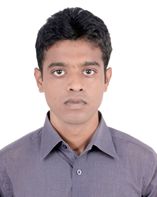
\includegraphics[width=\textwidth]{pic.jpg}
%\end{figure}}
%\end{minipage} % End the left-hand side of the page

\begin{minipage}[t]{0.44\textwidth} % Start the right-hand side of the page
\vspace{0pt} 
{\raggedright	
\colorbox{shade}{\textcolor{text1}{
\begin{tabular}{c|p{7cm}}
\raisebox{-4pt}{\textifsymbol{18}} & 353/A, Khilgaon, Tilpapara , Dhaka-1216 \\ % Address
\raisebox{-3pt}{\Mobilefone} & +880-01791693643 \\ % Phone number
\raisebox{-1pt}{\Letter} & \href{mailto:bitaron90@gmail.com}{bitaron90@gmail.com} \\ % Email address
%\Keyboard & \href{http://www.johnsmith.com}{http://www.johnsmith.com} \\ % Website
\end{tabular}
}
}\\[10pt]
}
\end{minipage}
%----------------------------------------------------------------------------------------
%	ABOUT ME
%----------------------------------------------------------------------------------------
%
%\section{About Me}
%\normalsize{Highly dependable Software Engineer and enthusiastic team player dedicated to streamlining processes and efficiently resolving project issues. Capable of applying design patterns to solve real world problems. Strongly motivated to use decoupled design architecture.}\\

%----------------------------------------------------------------------------------------
%	PRINCIPLES
%----------------------------------------------------------------------------------------
%
\section{Principles} 

\begin{tabular}{rl}
	\textsc{}
	& Clean Code. \\
	& Reliable and Reproducible Build System.\\
	& Feedback loop \\
	& Self testing Code base.\\
	& Separation of concerns. \\
	& Automate what you can. \\
	& Document everything. \\
\end{tabular}\\[10pt]


%----------------------------------------------------------------------------------------
%	EDUCATION
%----------------------------------------------------------------------------------------

\section{Education} 

\begin{tabular}{rl} % Start a table with two columns, one for dates and one for qualifications

%------------------------------------------------
% EDUCATION 1
%------------------------------------------------

2015 --  & \textbf{Bachelor of Science} \\ 
& \textsc{Computer Science and Engineering} \\ 
& \textit{Bangladesh University of Engineering and Technology}\\
& \textit{CGPA: 3.00/4}\\
	 

%----------------------------------------------------------------------------------------

\end{tabular}\\[10pt]

%----------------------------------------------------------------------------------------
%	COMPUTER SKILLS
%----------------------------------------------------------------------------------------

\section{Language Skill} 

\begin{tabular}{rl}
Intermediate 
& \textsc{java}, \textsc{javascript}, PHP, Shel ,SQL\\
&\\
Basic 
& \textsc{C family of languages}, \LaTeX, HTML \& css\\
\end{tabular}

%----------------------------------------------------------------------------------------
%	TOOL
%----------------------------------------------------------------------------------------

\section{Tools} 

\begin{tabular}{rl}
	
Intermediate
& Maven, Play, Node.js, React.js, Flux, jquery. \\
& Android, Gradle, Retrofit\\
& \\
Basic
& Angular.js, Laravel, Tomcat, AWS.\\
\end{tabular}\\[10pt]

%----------------------------------------------------------------------------------------
%	PERSONAL PROJECTS
%----------------------------------------------------------------------------------------
\section{Personal Projects} 


%------------------------------------------------
%	PROJECT 2
%------------------------------------------------


{\raggedright\large Build Systems \\
	\textit{\href {https://github.com/Bitaron/java-maven}{https://git.io/v15lc}(mvn), \href{https://github.com/Bitaron/java-sbt}{https://git.io/v15lW}(sbt)
		\href{https://github.com/Bitaron/js}{https://git.io/v15l4}(js)}\\[5pt]}
\textsc{- Use of \textbf{maven} with \textbf{JAX-RX} \& \textbf{JPA}. }\\
\textsc{- Use of \textbf{sbt} with \textbf{Play} \& \textbf{Ebean}..}\\
\textsc{- Build system using \textbf{node} and \textbf{jake}}\\
\normalsize{}\\


%------------------------------------------------
%	PROJECT 4
%------------------------------------------------


{\raggedright\large Weather Application \\
	\textit{\href {https://github.com/Bitaron/js/tree/weather}{https://git.io/v15lR}}\\[5pt]}
\textsc{- Display temperature and current local time based on city.}\\
\textsc{- Use of \textbf{react.js} and \textbf{flux} architecture.}\\
\textsc{- Testing \textbf{flux} using \textbf{jasmine}.}\\


%%------------------------------------------------
%%	PROJECT 5
%%------------------------------------------------
%
%
{\raggedright\large Android Applications \\
	\textit{\href {https://www.dropbox.com/s/3qdujsilwmpq720/letsgo.apk?dl=0}{https://bit.ly/2Kkv8Z6}}\\[5pt]}
	\textsc{- Turn mobile silent based on predefined time and \textbf{geofence}.}\\
\textsc{- Use of \textbf{gradle}.}\\
%		\textit{Lets Go \href {https://dl.dropboxusercontent.com/u/84146203/projects/android/letsgo.apk}{http://bit.ly/2hwlipz}}\\[5pt]
%		\textsc{- List nearby places based on users location and preference}\\
%\textsc{- Use of \textbf{node-express-mongo} stack}\\
%\textsc{- Use of \textbf{retrofit},\textbf{android account} \& \textbf{google map}}\\




%----------------------------------------------------------------------------------------

	
\end{minipage} % End right-hand side of the page

\end{document}  